\documentclass{article}
\usepackage{tkz-graph}
\usepackage{paralist}
\pagestyle{empty}
\usetikzlibrary{patterns}

\newcommand{\align}[1]{
	\begingroup
	\setbox0=\hbox{#1}
	\parbox{\wd0}{\box0}\endgroup
}

\begin{document}

\makebox[5cm]{{\bf 5x with no diagonal}}
\align{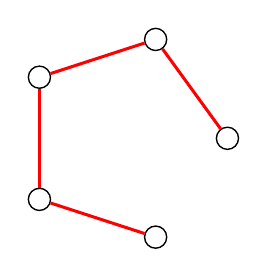
\begin{tikzpicture}[scale=0.66]

\GraphInit[vstyle=Simple]

\SetUpEdge[lw = 1.1pt, color = red]
\tikzset{VertexStyle/.append style = {minimum size = 8pt, inner sep = 0pt, fill=white}}    

\Vertices[unit=2]{circle}{1,2,3,4,5}

\Edges(1,2,3,4,5)

\end{tikzpicture}}

\makebox[5cm]{{\bf 2x5x with one diagonal}}
\align{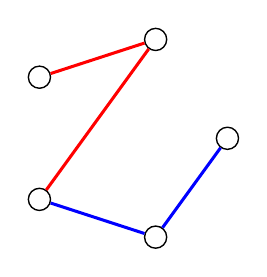
\begin{tikzpicture}[scale=0.66]

\GraphInit[vstyle=Simple]

\SetUpEdge[lw = 1.1pt, color = red]
\tikzset{VertexStyle/.append style = {minimum size = 8pt, inner sep = 0pt, fill=white}}    

\Vertices[unit=2]{circle}{1,2,3,4,5}

\Edges(3,2,4)
\SetUpEdge[lw = 1.1pt, color = blue]
\Edges(4,5,1)

\end{tikzpicture}
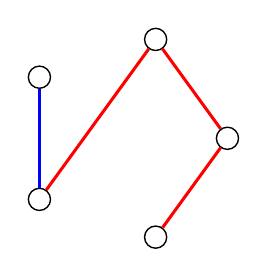
\begin{tikzpicture}[scale=0.66]

\GraphInit[vstyle=Simple]

\SetUpEdge[lw = 1.1pt, color = red]
\tikzset{VertexStyle/.append style = {minimum size = 8pt, inner sep = 0pt, fill=white}}    

\Vertices[unit=2]{circle}{1,2,3,4,5}

\Edges(5,1,2,4)
\SetUpEdge[lw = 1.1pt, color = blue]
\Edges(4,3)

\end{tikzpicture}}

\makebox[5cm]{{\bf 5x with two diagonals}}
\align{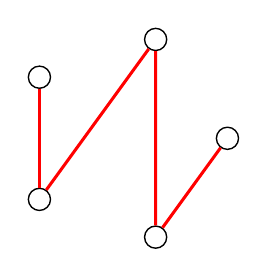
\begin{tikzpicture}[scale=0.66]

\GraphInit[vstyle=Simple]

\SetUpEdge[lw = 1.1pt, color = red]
\tikzset{VertexStyle/.append style = {minimum size = 8pt, inner sep = 0pt, fill=white}}    

\Vertices[unit=2]{circle}{1,2,3,4,5}

\Edges(3,4,2,5,1)

\end{tikzpicture}}

\end{document}